Here we discuss the implementation of the experimental system to prove the concept of our proposed load balancers with ECMP redundancy in detail.

\section{Experimental system architecture}

\begin{figure}[tb]
\begin{center}
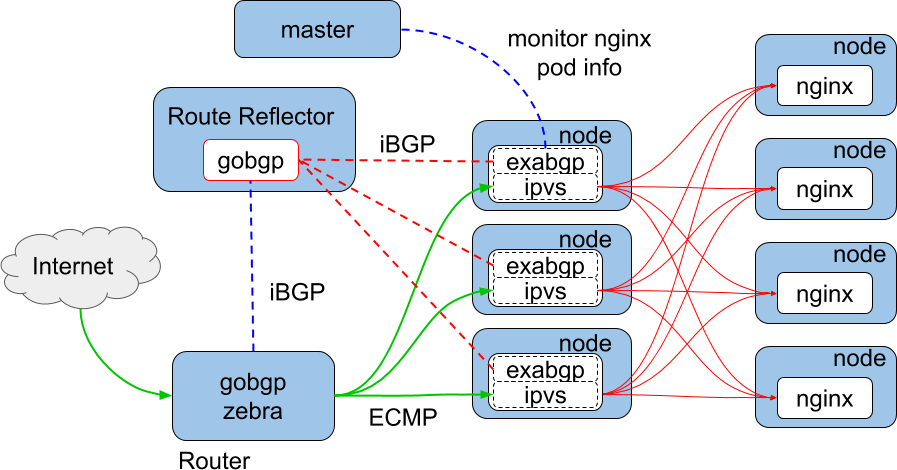
\includegraphics[width=0.8\columnwidth]{Figs/poc.png}
\end{center}
\caption{
  An experimental container cluster with proposed redundant software balancers. \\ %\par 
  The master and nodes are configured as Kubernetes's master and nodes on top of conventional Linux boxes, respectively.
  The route reflector and the upstream router are also conventional Linux boxes.
}
\label{fig:poc}
\end{figure}

Fig.~\ref{fig:poc} shows the schematic diagram of proof of concept container cluster system with our proposed redundant software load balancers.
All the nodes and route reflector are configured using Debian 9.5 with self compiled linux-4.16.12 kernel.  
The upstream router also used conventional linux box using the same OS as the nodes and route reflector.
For the Linux kernel to support hash based ECMP routing table we needed to use kernel version 4.12 or later.
We also needed to enable kernel config option CONFIG\_IP\_ROUTE\_MULTIPATH\cite{ip-sysctl} when compiling, and set the kernel parameter fib\_multipath\_hash\_policy=1 at run time.
In the actual production environment, proprietary hardware with the highest throughput is often deployed, but we could still test some of the required advanced functions by using a Linux box.

Each load balancer pod consists of an exabgp container and an ipvs container.
The ipvs container is responsible for distributing the traffic toward the IP address that a service uses, to web(nginx) server pods.
The ipvs container monitors the availability of web server pods and manages the load balancing rule appropriately.
The exabgp container is responsible for advertising the route toward the IP address that a service uses, to the route reflector.
The route reflector aggregates the routing information advertised by load balancer pods and advertise them to the upstream router.

The exabgp is used in the load balancer pods because of the simplicity in setting as static route advertiser.
On the other hand, gobgp is used in the router and the route reflector, because exabgp did not seem to support add-path\cite{rfc7911} needed for multi-path advertisement and Forwarding Information Base(FIB) manipulation\cite{exa-networks_2018}.
The gobgp supports the add-path, and the FIB manipulation through zebra\cite{osrg_gobgp_zebra}.
The configurations for the router is summarised in \ref{appendix:router_config}.

The route reflector also uses a Linux box with gobgp and overlay network setup.
The requirements for the BGP agent on the route reflector are dynamic-neighbours and add-paths features.
The configurations for the route reflector is summarised in \ref{appendix:route_reflector_config}.

\section{Ipvs container}

\begin{figure}
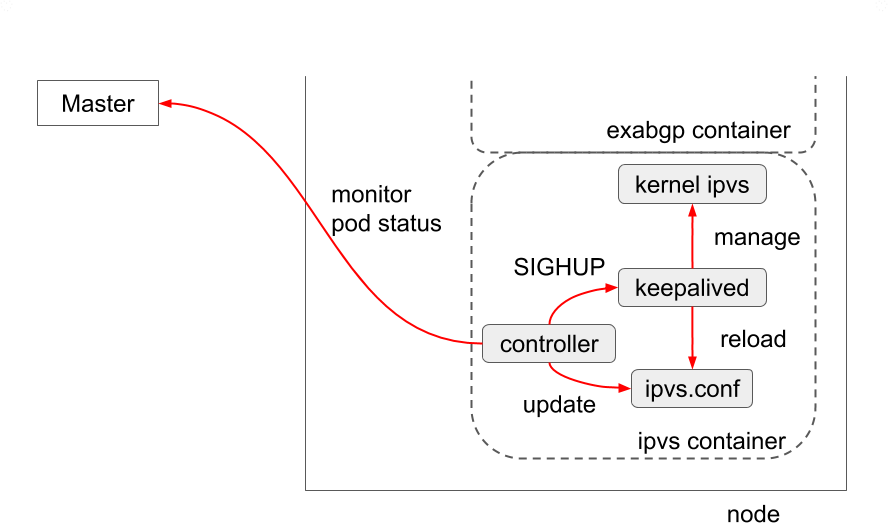
\includegraphics[width=0.8\columnwidth]{Figs/ipvs-ingress-schem}
\caption{Implementation}
\label{fig:IPVS-ingress-schem}
\end{figure}

The proposed load balancer needs to dynamically reconfigure the IPVS balancing rules whenever {\em pods} are created/deleted. 
Figure~\ref{fig:IPVS-ingress-schem} is a schematic diagram to show the dynamic reconfiguration of the IPVS rules.
The right part of the figure shows the enlarged view of one of the nodes where the load balancer pod(LB2) is deployed.
Two daemon programs, controller and keepalived, run in the container inside the LB2 pod are illustrated.
The keepalived manages Linux kernel's IPVS rules depending on the ipvs.conf configuration file.
It is also capable of health-checking the liveliness of {\em real server}, 
which is represented as a combination of the IP addresses and port numbers of the target {\em pods}. 
If the health check to a {\em real server} fails, keepalived will remove that {\em real server} from the IPVS rules.

The controller monitors information concerning the running {\em pods} of a service 
in the Kubernetes cluster by consulting the apiserver running on the master.
Whenever {\em pods} are created or deleted, the controller will automatically regenerate an appropriate ipvs.conf 
and issue SIGHUP to keepalived.
Then, keepalived will reload the ipvs.conf and modify the kernel's IPVS rules accordingly.
The actual controller\cite{ktaka_ccmp_2017_826894} is implemented using the Kubernetes ingress controller\cite{K8sIngress2017} framework. 
By importing existing Golang package, \enquote{k8s.io/ingress /core/pkg/ingress}, we could simplify the implementation, e.g. 
120 lines of code.  

%In this way, the IPVS's balancing rules inside Linux kernel are maintained so that it can distribute the incoming traffic only to the living pods.

Configurations for capabilities were needed in the implementation: adding the CAP\_SYS\_MODULE capability 
to the container to allow the kernel to load required kernel modules inside a container, 
and adding CAP\_NET\_ADMIN capability to the container to allow keepalived to manipulate the kernel's IPVS rules. 
For the former case, we also needed to mount the \enquote{/lib/module} of the node's file system on the container's file system.

\begin{figure}
  \centering
\begin{minipage}{0.7\columnwidth}
\begin{lstlisting}[frame=single]
  virtual_server fwmark 1 {
    delay_loop 5
    lb_algo lc
    lb_kind NAT
    protocol TCP
    real_server 172.16.21.2 80 {
      uthreshold 20000
      TCP_CHECK {
        connect_timeout 5
        connect_port 80
      }
    }
    real_server 172.16.80.2 80 {
      uthreshold 20000
      TCP_CHECK {
        connect_timeout 5
        connect_port 80
      }
    }
  }
\end{lstlisting}
\end{minipage}
\caption{An example of ipvs.conf}
\label{fig:ipvs.conf}
\end{figure}

\begin{figure}
  \centering
%\begin{minipage}{\columnwidth}
\rule{\columnwidth}{0.4pt}
\begin{verbatim}
# kubectl exec -it IPVS-controller-4117154712-kv633 -- IPVSadm -L
IP Virtual Server version 1.2.1 (size=4096)
Prot LocalAddress:Port Scheduler Flags
  -> RemoteAddress:Port Forward Weight ActiveConn InActConn
FWM  1 lc
  -> 172.16.21.2:80      Masq    1      0          0         
  -> 172.16.80.2:80      Masq    1      0          0
\end{verbatim}
\rule{\columnwidth}{0.4pt}
%\end{minipage}
\caption{Example of IPVS balancing rules}
\label{fig:IPVS rule}
\end{figure}


Figure~\ref{fig:ipvs.conf} and Figure~\ref{fig:IPVS rule} show an example of an ipvs.conf file 
generated by the controller and the corresponding IPVS load balancing rules, respectively.
Here, we can see that the packet with {\tt fwmark=1}\cite{BertHubert2002} is distributed 
to {\tt 172.16.21.2:80} and {\tt 172.16.80.2:80} 
using the masquerade mode(Masq) and 
the least connection(lc)\cite{Zhang2000} balancing algorithm.


\section{BGP software container}

\begin{figure}[tb]

  \begin{subfigure}[t]{\columnwidth}
    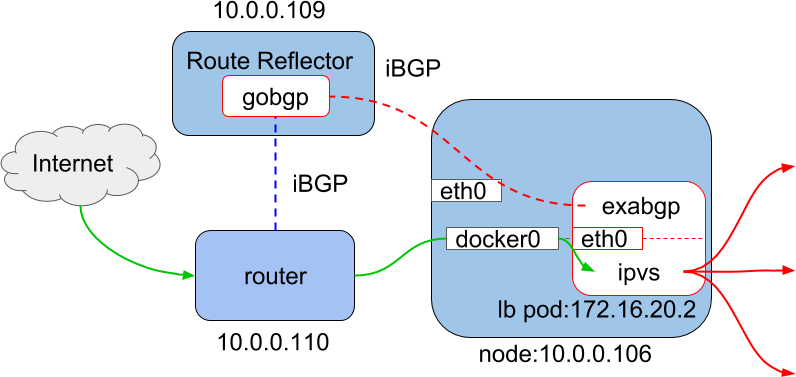
\includegraphics[width=0.9\columnwidth]{Figs/exabgp}
    \caption{}
    \label{fig:exabgp_schem}
  \end{subfigure}

  \par\bigskip

  \begin{subtable}{.9\textwidth}
    \centering
    \begin{tabular}{l}
      \hline 
      \multicolumn{1}{l}{[BGP announcement]} \\
      \hspace{15 mm} route 10.1.1.0/24 next-hop 10.0.0.106 \\
      \multicolumn{1}{l}{[Routing in node net namespace]} \\
      \hspace{15 mm} ip netns exec node ip route replace 10.1.1.0/24 dev docker0 \\
      \multicolumn{1}{l}{[Accept as local]} \\
      \hspace{15 mm} ip route add local 10.1.1.0/24 dev eth0 \\
      \hline
    \end{tabular}
    \caption{}
    \label{tab:single}
  \end{subtable}

  \caption{
    (a) Network path by the exabgp container. (b) Required settings in the exabgp container.
  }
  \label{fig:exabgp}
\end{figure}

In order to implement the ECMP redundancy, we also containerized exabgp using Docker.
Fig.\ref{fig:exabgp}~(\subref{fig:exabgp_schem}) shows a schematic diagram of the network path realized by the exabgp container.
We used exabgp as the BGP advertiser as mentioned earlier.
The traffic from the Internet is forwarded by ECMP routing table on the router to the node, then routed to ipvs container.

Fig.\ref{fig:exabgp}~(\subref{fig:exabgp_setting}) summarises some key settings required for the exabgp container.
In BGP announcements the node IP address, 10.0.0.106 is used as the next-hop for the IP range 10.1.1.0/24.
Then on the node, in order to route the packets toward 10.1.1.0/24 to the ipvs container, 
a routing rule to the dev docker0 is created in the node net namespace. 
A routing rule to accept the packets toward those IPs as local is also required in the container net namespace. 
A configuration of exabgp is shown in \ref{appendix:exabgp_config}.

\section{ingress controller}

\section{choice bgp software}

